\chapter{中央处理器}\label{CO05}

\section{CPU 功能、寄存器与状态元件}\label{CO05-state}

CPU完成指令控制、操作控制、时间控制、数据加工及规定的异常/中断处理。数据通路完成数据传送和运算，控制部件CU生成选择、运算、写使能与存储器读写等控制信号。

\par\smallskip
{\fontsize{9.3}{12}\selectfont\setlength{\tabcolsep}{2.5pt}\setlength{\LTleft}{0pt}\setlength{\LTright}{0pt}
\begin{longtable}{@{}>{\raggedright\arraybackslash}p{\dimexpr0.31295\linewidth-2\tabcolsep\relax}>{\raggedright\arraybackslash}p{\dimexpr0.39042\linewidth-2\tabcolsep\relax}>{\raggedright\arraybackslash}p{\dimexpr0.29664\linewidth-2\tabcolsep\relax}@{}}
\toprule
部件 & 内容或作用 & 组织层次 \\

\midrule\endfirsthead\toprule
部件 & 内容或作用 & 组织层次 \\

\midrule\endhead\bottomrule\endfoot
ALU、MUX、移位器 & 按当前输入形成运算或选择结果 & 组合逻辑操作元件 \\

GPRs、ACC、临时寄存器 & 操作数、地址、中间结果 & 状态元件 \\

PC & 程序执行位置，更新规则依ISA与时序 & 程序级状态 \\

IR & 当前指令编码 & 通常属实现内部 \\

MAR & 本次主存访问地址 & 通常属实现内部 \\

MDR & 本次与主存交换的指令或数据 & 通常属实现内部 \\

PSW/FR & 条件码及规定的特权、中断等状态 & 可见性与写权限依ISA \\

CMAR、CMDR & 微地址、当前微指令 & 微程序控制器内部 \\

\end{longtable}}
\par\smallskip

GPRs、PC及规定的状态属于程序员可见模型；可见性与用户指令能否直接读写分别由ISA及权限定义。MAR位数按可寻址单元数确定，MDR位数按一次数据交换位宽确定。例如26位字节地址、32位数据通路，可有26位MAR与32位MDR。

\par\medskip\Needspace{4\baselineskip}\noindent\hypertarget{CO05-E01}{}\label{CO05-E01}\textbf{例 5-1}\par\nobreak\smallskip

数据通路由组合逻辑元件（操作元件）和时序逻辑元件（状态元件）组成。以下给出的元件中，属于操作元件的是（　）。

I. 算术逻辑部件（ALU）　II. 程序计数器（PC）\\
III. 通用寄存器组（GPRs）　IV. 多路选择器（MUX）

A. 仅 I、II　 B. 仅 I、IV　 C. 仅 II、III　 D. 仅 I、II、IV

\section{指令周期与三种执行组织}\label{CO05-cycle-model}

指令周期覆盖一条指令从开始到完成；机器周期为某实现划分的访存等基本操作周期；时钟周期为同步状态推进的时间单位。三者倍数由具体组织给出。

\par\smallskip
{\fontsize{9.3}{12}\selectfont\setlength{\tabcolsep}{2.5pt}\setlength{\LTleft}{0pt}\setlength{\LTright}{0pt}
\begin{longtable}{@{}>{\raggedright\arraybackslash}p{\dimexpr0.22422\linewidth-2\tabcolsep\relax}>{\raggedright\arraybackslash}p{\dimexpr0.42127\linewidth-2\tabcolsep\relax}>{\raggedright\arraybackslash}p{\dimexpr0.35452\linewidth-2\tabcolsep\relax}@{}}
\toprule
指令阶段 & 动作 & 进入条件 \\

\midrule\endfirsthead\toprule
指令阶段 & 动作 & 进入条件 \\

\midrule\endhead\bottomrule\endfoot
取指 & PC给地址、读指令入IR、更新PC & 每条指令 \\

间址 & 取得有效地址 & 需要主存间接寻址等 \\

执行 & 完成指令语义 & 每条指令，动作不同 \\

中断 & 保存返回状态、进入处理入口 & 有请求且满足响应条件 \\

\end{longtable}}
\par\smallskip

\par\smallskip
{\fontsize{9.3}{12}\selectfont\setlength{\tabcolsep}{2.5pt}\setlength{\LTleft}{0pt}\setlength{\LTright}{0pt}
\begin{longtable}{@{}>{\raggedright\arraybackslash}p{\dimexpr0.24478\linewidth-2\tabcolsep\relax}>{\raggedright\arraybackslash}p{\dimexpr0.30833\linewidth-2\tabcolsep\relax}>{\raggedright\arraybackslash}p{\dimexpr0.44690\linewidth-2\tabcolsep\relax}@{}}
\toprule
组织 & 时钟约束 & 同一时刻与资源复用 \\

\midrule\endfirsthead\toprule
组织 & 时钟约束 & 同一时刻与资源复用 \\

\midrule\endhead\bottomrule\endfoot
单周期 & 最慢完整指令路径 & 一条指令占一长拍；同拍资源需求须同时满足 \\

多周期 & 最慢基本步骤 & 一条指令分多拍；资源可跨拍复用 \\

简单标量流水 & 最慢段+段寄存器开销 & 多条指令不同段重叠；同拍资源争用须消除 \\

\end{longtable}}
\par\smallskip

单周期CPI=1、理想标量流水稳态CPI约1，周期长度可不同。性能比较用执行时间 \(N\times\mathrm{CPI}\times\tau\)。

\section{单总线数据通路与微操作时序}\label{CO05-bus-operations}

微操作是部件可执行的基本动作；微命令为驱动该动作的控制命令。同一内部总线每拍通常只允许一个驱动源，多个目的在有实际通路和独立写使能时可同时接收同一值。

ALU一端由Y保存第一个操作数，另一端接总线；结果先存Z，后续再上总线写回。例 \(R_1\leftarrow R_1+R_2\)：

\par\smallskip
{\fontsize{9.3}{12}\selectfont\setlength{\tabcolsep}{2.5pt}\setlength{\LTleft}{0pt}\setlength{\LTright}{0pt}
\begin{longtable}{@{}>{\raggedright\arraybackslash}p{\dimexpr0.36680\linewidth-2\tabcolsep\relax}>{\raggedright\arraybackslash}p{\dimexpr0.63320\linewidth-2\tabcolsep\relax}@{}}
\toprule
拍 & 微操作 \\

\midrule\endfirsthead\toprule
拍 & 微操作 \\

\midrule\endhead\bottomrule\endfoot
1 & \(R_1\to Y\) \\

2 & \(R_2\to\mathrm{BUS}\)，\(Y+\mathrm{BUS}\to Z\) \\

3 & \(Z\to R_1\) \\

\end{longtable}}
\par\smallskip

\texttt{R1→Y}与\texttt{R2→MAR}同拍争用总线；\texttt{R1→Y}与\texttt{R1→MAR}可同时接收。结果尚未产生、访存尚未完成时，目的寄存器应等待。

取指依赖：\(\mathrm{PC}\to\mathrm{MAR}\)，主存读入MDR，\(\mathrm{MDR}\to\mathrm{IR}\)；指令地址字段需间接求址时，再送MAR并读出有效地址。PC增量能否与访存并行取决于独立增量器、总线占用与图示通路。

\par\medskip\Needspace{4\baselineskip}\noindent\hypertarget{CO05-E02}{}\label{CO05-E02}\textbf{例 5-2}\par\nobreak\smallskip

某CPU中部分数据通路如下图所示，其中，GPRs为通用寄存器组；FR为标志寄存器，用于存放ALU产生的标志信息；带箭头虚线表示控制信号，如控制信号Read、Write分别表示主存读、主存写，MDRin表示内部总线上数据写入MDR，MDRout表示MDR的内容送内部总线。

\begin{figure}[H]
\centering
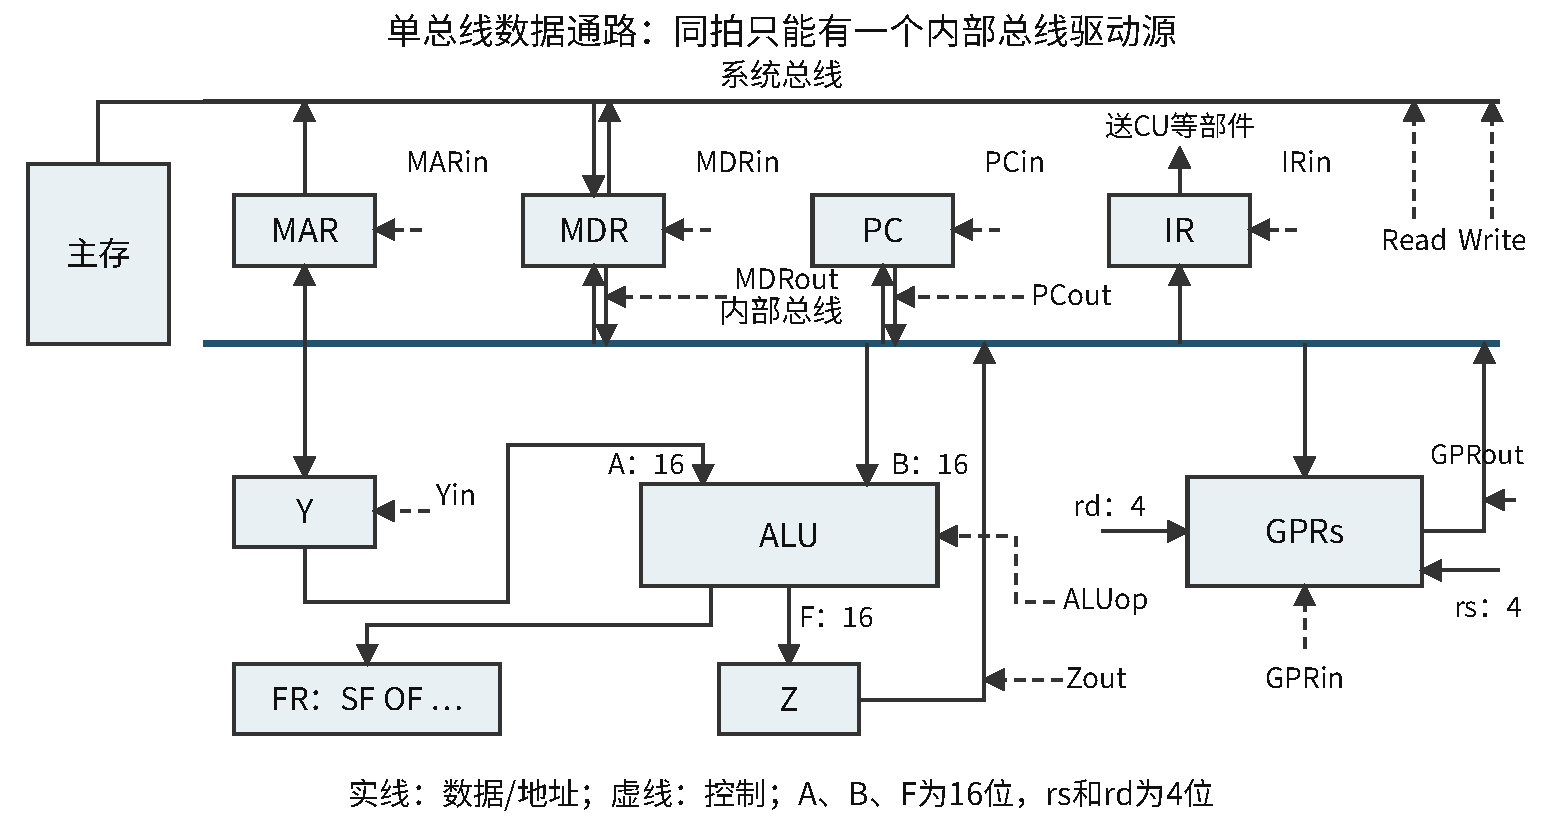
\includegraphics[width=\linewidth,height=108mm,keepaspectratio]{figures/CO_F07_datapath.pdf}
\caption{单条内部总线连接Y、ALU与Z；rs、rd为4位寄存器编号}\label{co-fig-datapath}
\end{figure}

（1）设ALU的输入端A、B及输出端F的最高位分别为A15、B15及F15，FR中的符号标志和溢出标志分别为SF和OF，则SF的逻辑表达式是什么？A加B、A减B时OF的逻辑表达式分别是什么？要求逻辑表达式的输入变量为A15、B15及F15。

（2）为什么要设置暂存器Y和Z？

（3）若GPRs的输入端rs、rd分别为所读、写的通用寄存器的编号，则GPRs中最多有多少个通用寄存器？rs和rd来自图中的哪个寄存器？已知GPRs内部有一个地址译码器和一个多路选择器，rd应连接地址译码器还是多路选择器？

（4）取指令阶段（不考虑PC增量操作）的控制信号序列是什么？若从发出主存读命令到主存读出数据并传送到MDR共需5个时钟周期，则取指令阶段至少需要几个时钟周期？

（5）图中控制信号由什么部件产生？图中哪些寄存器的输出信号会连到该部件的输入端？

\par\medskip\Needspace{4\baselineskip}\noindent\hypertarget{CO05-E03}{}\label{CO05-E03}\textbf{例 5-3}\par\nobreak\smallskip

某指令功能为 \(\mathrm R[r2]\leftarrow\mathrm R[r1]+\mathrm M[\mathrm R[r0]]\)，其两个源操作数分别采用寄存器、寄存器间接寻址方式。对于下列给定部件，该指令在取数及执行过程中需要用到的是（　）。

I. 通用寄存器组（GPRs）　II. 算术逻辑单元（ALU）\\
III. 存储器（Memory）　IV. 指令译码器（ID）

A. 仅 I、II　 B. 仅 I、II、III　 C. 仅 II、III、IV　 D. 仅 I、III、IV

\section{硬布线与微程序控制器}\label{CO05-controller}

\par\smallskip
\begin{wideblock}
{\fontsize{9.3}{12}\selectfont\setlength{\tabcolsep}{2.5pt}\setlength{\LTleft}{0pt}\setlength{\LTright}{0pt}
\begin{longtable}{@{}>{\raggedright\arraybackslash}p{\dimexpr0.20440\linewidth-2\tabcolsep\relax}>{\raggedright\arraybackslash}p{\dimexpr0.38240\linewidth-2\tabcolsep\relax}>{\raggedright\arraybackslash}p{\dimexpr0.41320\linewidth-2\tabcolsep\relax}@{}}
\toprule
维度 & 硬布线控制 & 微程序控制 \\

\midrule\endfirsthead\toprule
维度 & 硬布线控制 & 微程序控制 \\

\midrule\endhead\bottomrule\endfoot
控制信号来源 & 操作码、节拍、周期状态及标志经逻辑电路形成 & 控存微指令的控制字段直接或译码形成 \\

常见特点 & 控制延迟较短；修改复杂功能需改逻辑 & 便于组织复杂控制；受控存与微周期开销影响 \\

设计步骤 & 列微操作→排节拍→合成控制逻辑 & 列微操作/节拍→选编码与下址方式→分配控存→编微码 \\

\end{longtable}}
\end{wideblock}
\par\smallskip

硬布线中某信号在指令A的\(T_1\)或指令B的\(T_2\)发生，可写 \(C=A\cdot T_1+B\cdot T_2\)；加、乘分别为逻辑或、与，条件标志乘入相应项。

\par\smallskip
{\fontsize{9.3}{12}\selectfont\setlength{\tabcolsep}{2.5pt}\setlength{\LTleft}{0pt}\setlength{\LTright}{0pt}
\begin{longtable}{@{}>{\raggedright\arraybackslash}p{\dimexpr0.37033\linewidth-2\tabcolsep\relax}>{\raggedright\arraybackslash}p{\dimexpr0.62967\linewidth-2\tabcolsep\relax}@{}}
\toprule
微程序对象 & 含义 \\

\midrule\endfirsthead\toprule
微程序对象 & 含义 \\

\midrule\endhead\bottomrule\endfoot
机器指令 & ISA规定的一次软件可见操作 \\

微程序 & 实现一条机器指令等功能的微指令序列 \\

微指令 & 一个微周期的操作控制和顺序控制信息 \\

微命令 & 使具体部件执行微操作的控制信号 \\

CM/CMAR/CMDR & 控制存储器/微地址寄存器/微指令寄存器 \\

\end{longtable}}
\par\smallskip

PC、MAR对应机器程序/主存空间；CMAR定位控存。公共取指微程序可共享，取指结束由IR操作码映射执行入口，执行结束回取指入口。间址、中断等可有公共段；入口具体地址依模型规定。

\begin{figure}[H]
\centering
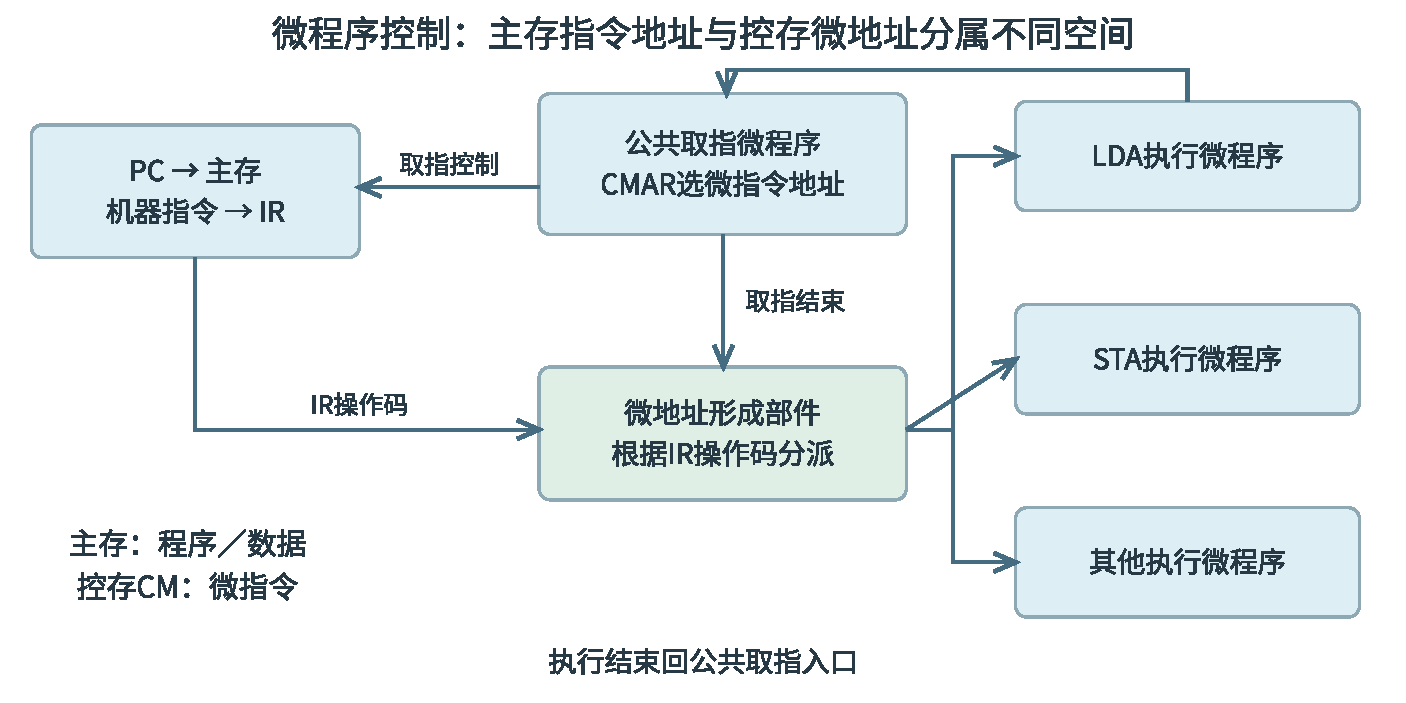
\includegraphics[width=\linewidth,height=108mm,keepaspectratio]{figures/CO05_microprogram_flow.pdf}
\caption{取指入口、操作码映射和执行微程序}
\end{figure}

\par\smallskip
{\fontsize{9.3}{12}\selectfont\setlength{\tabcolsep}{2.5pt}\setlength{\LTleft}{0pt}\setlength{\LTright}{0pt}
\begin{longtable}{@{}>{\raggedright\arraybackslash}p{\dimexpr0.31002\linewidth-2\tabcolsep\relax}>{\raggedright\arraybackslash}p{\dimexpr0.68998\linewidth-2\tabcolsep\relax}@{}}
\toprule
控制字段编码 & 位数与并行性 \\

\midrule\endfirsthead\toprule
控制字段编码 & 位数与并行性 \\

\midrule\endhead\bottomrule\endfoot
直接控制 & 每个微命令一位；宽、译码简单、并行性强 \\

字段直接编码 & 互斥微命令同组，各组可并行；含\(k\)条命令及空操作需\(\lceil\log_2(k+1)\rceil\)位 \\

字段间接编码 & 利用字段间依赖解释；进一步压缩并增加译码层次 \\

\end{longtable}}
\par\smallskip

水平型通常控制字较宽、并行微操作较多；垂直型编码较强、字短，可能需更多微指令；混合型折中。下微地址可来自下地址字段、顺序增量、操作码映射、条件测试或硬件强制入口。控存含\(M\)个可区分地址时，地址至少\(\lceil\log_2M\rceil\)位。

静态微程序通常固化于ROM；动态微程序使用可改写控存；毫微程序在微指令之下再设解释层。修改能力取决于硬件支持。

\par\medskip\Needspace{4\baselineskip}\noindent\hypertarget{CO05-E04}{}\label{CO05-E04}\textbf{例 5-4}\par\nobreak\smallskip

某计算机的控制器采用微程序控制方式，微指令中的操作控制字段采用字段直接编码法，共有33个微命令，构成5个互斥类，分别包含7、3、12、5和6个微命令，则操作控制字段至少有（　）。

A. 5位　 B. 6位　 C. 15位　 D. 33位

\par\medskip\Needspace{4\baselineskip}\noindent\hypertarget{CO05-E05}{}\label{CO05-E05}\textbf{例 5-5}\par\nobreak\smallskip

某计算机采用微程序控制器，共有32条指令，公共的取指令微程序包含2条微指令，各指令对应的微程序平均由4条微指令组成，采用断定法（下地址字段法）确定下条微指令地址，则微指令中下地址字段的位数至少是（　）。

A. 5　 B. 6　 C. 8　 D. 9

\section{异常、中断与返回断点}\label{CO05-events}

\par\smallskip
{\fontsize{9.3}{12}\selectfont\setlength{\tabcolsep}{2.5pt}\setlength{\LTleft}{0pt}\setlength{\LTright}{0pt}
\begin{longtable}{@{}>{\raggedright\arraybackslash}p{\dimexpr0.30830\linewidth-2\tabcolsep\relax}>{\raggedright\arraybackslash}p{\dimexpr0.40038\linewidth-2\tabcolsep\relax}>{\raggedright\arraybackslash}p{\dimexpr0.29132\linewidth-2\tabcolsep\relax}@{}}
\toprule
事件 & 检测与处理 & 常见返回位置 \\

\midrule\endfirsthead\toprule
事件 & 检测与处理 & 常见返回位置 \\

\midrule\endhead\bottomrule\endfoot
故障fault，如缺页 & 当前指令未完成；修复后重试 & 当前指令起点 \\

陷阱trap，如系统调用 & 执行有意通知/服务请求 & 通常为后继位置 \\

终止abort & 严重异常，通常无法可靠恢复 & 依体系结构 \\

外部中断 & 设备、定时器等；通常在指令边界响应 & 下一条尚未执行指令 \\

\end{longtable}}
\par\smallskip

具体分类、保存PC及可恢复规则由ISA确定。硬件响应保存规定的断点与处理器状态、切换状态并进入入口；软件继续保存所需通用寄存器现场。``中断隐指令''为硬件响应动作的教材称呼。中断服务程序为软件。

\begin{figure}[H]
\centering
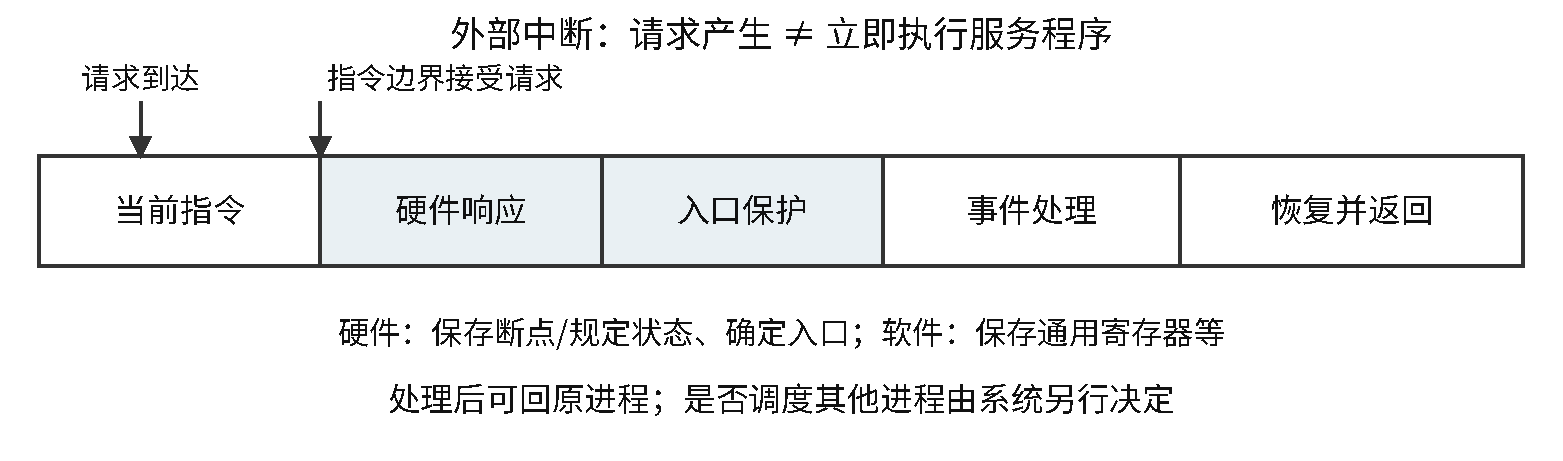
\includegraphics[width=\linewidth,height=108mm,keepaspectratio]{figures/CO_F08_interrupt_response.pdf}
\caption{外部请求、硬件入口与软件处理}
\end{figure}

进入内核态后可返回原进程，也可由调度器切换进程；模式切换与上下文切换分开判断。

\par\medskip\Needspace{4\baselineskip}\noindent\hypertarget{CO05-E06}{}\label{CO05-E06}\textbf{例 5-6}\par\nobreak\smallskip

异常事件在当前指令执行过程中进行检测，中断请求则在当前指令执行后进行检测。下列事件中，相应处理程序执行后，必须回到当前指令重新执行的是（　）。

A. 系统调用　 B. 页缺失　 C. DMA传送结束　 D. 打印机缺纸

\section{流水线阶段、时钟与性能公式}\label{CO05-pipeline}

\par\smallskip
{\fontsize{9.3}{12}\selectfont\setlength{\tabcolsep}{2.5pt}\setlength{\LTleft}{0pt}\setlength{\LTright}{0pt}
\begin{longtable}{@{}>{\raggedright\arraybackslash}p{\dimexpr0.36917\linewidth-2\tabcolsep\relax}>{\raggedright\arraybackslash}p{\dimexpr0.63083\linewidth-2\tabcolsep\relax}@{}}
\toprule
阶段 & 典型工作 \\

\midrule\endfirsthead\toprule
阶段 & 典型工作 \\

\midrule\endhead\bottomrule\endfoot
IF & 取指 \\

ID & 译码、读源寄存器 \\

EX & ALU运算、计算有效地址 \\

MEM & LOAD读数据、STORE写数据 \\

WB & 写回寄存器 \\

\end{longtable}}
\par\smallskip

ALU结果在EX末形成，LOAD数据通常在MEM末形成；STORE通常无寄存器写回。固定五段题可要求所有指令流出五段后才计完成。阶段寄存器须携带数据、立即数、目的寄存器号、控制位、指令地址和必要异常信息。

冻结保持原有状态；气泡是不会改变有效状态的空操作。二者须配合写使能，避免重复写入或错误访存。

等时\(k\)段、时钟\(\tau\)、每拍启动一条、无冒险时：

\[
T=(k+n-1)\tau,\quad \mathrm{TP}=\frac{n}{T},\quad
S=\frac{nk}{k+n-1},\quad E=\frac{n}{k+n-1}.
\]

\(S\)以非流水每条耗\(k\tau\)为基线；\(E\)假定每条有效使用全部\(k\)段。实际有用面积、原机器周期不同须重新计算。整体延长\(s\)拍时，\(T=(k+n-1+s)\tau\)。\(\tau\ge\max t_i+t_r\)，\(t_r\)为段寄存器开销；单条延迟约\(k\tau\)，稳态完成间隔为\(\tau\)。

\par\medskip\Needspace{4\baselineskip}\noindent\hypertarget{CO05-E07}{}\label{CO05-E07}\textbf{例 5-7}\par\nobreak\smallskip

某计算机的指令流水线由四个功能段组成，指令流经各功能段的时间（忽略各功能段之间的缓存时间）分别为90 ns、80 ns、70 ns和60 ns，则该计算机的 CPU 时钟周期至少是（　）。

A. 90 ns　 B. 80 ns　 C. 70 ns　 D. 60 ns

按层次分部件级、处理机级、处理机间流水；按功能分单/多功能；按同一时刻功能配置分静态/动态；按有无反馈分线性/非线性。动态流水线的功能分类与指令动态调度分别判断。

\section{结构、数据与控制冒险}\label{CO05-hazard}

\par\smallskip
{\fontsize{9.3}{12}\selectfont\setlength{\tabcolsep}{2.5pt}\setlength{\LTleft}{0pt}\setlength{\LTright}{0pt}
\begin{longtable}{@{}>{\raggedright\arraybackslash}p{\dimexpr0.29312\linewidth-2\tabcolsep\relax}>{\raggedright\arraybackslash}p{\dimexpr0.70688\linewidth-2\tabcolsep\relax}@{}}
\toprule
类别 & 冲突及处理 \\

\midrule\endfirsthead\toprule
类别 & 冲突及处理 \\

\midrule\endhead\bottomrule\endfoot
结构冒险 & 同拍争用不足的资源；停顿、加端口、分离指令/数据存储器 \\

RAW写后读 & 消费者需前指令新值；等待、转发、合法指令调度 \\

WAR读后写 & 后写覆盖尚未读取的旧值；重命名可消除名字冲突 \\

WAW写后写 & 两次写完成次序改变最终值；重命名、按序提交 \\

控制冒险 & 条件或后继目标未定；阻塞、预测、合法调度 \\

\end{longtable}}
\par\smallskip

固定五段、顺序发射、ID读且WB顺序写的简单模型通常只需处理RAW；乱序或不同延迟写回可能产生WAR/WAW。无条件转移在目标尚未获得时也可能造成控制冒险。

\par\smallskip
{\fontsize{9.3}{12}\selectfont\setlength{\tabcolsep}{2.5pt}\setlength{\LTleft}{0pt}\setlength{\LTright}{0pt}
\begin{longtable}{@{}>{\raggedright\arraybackslash}p{\dimexpr0.44218\linewidth-2\tabcolsep\relax}>{\raggedright\arraybackslash}p{\dimexpr0.55782\linewidth-2\tabcolsep\relax}@{}}
\toprule
时序/旁路条件 & 消费者最早可用时刻 \\

\midrule\endfirsthead\toprule
时序/旁路条件 & 消费者最早可用时刻 \\

\midrule\endhead\bottomrule\endfoot
无转发，同寄存器不能同拍读写 & ID晚于生产者WB至少1拍 \\

无转发，同拍先写后读 & ID可与生产者WB同拍 \\

EX结果向EX转发 & 生产者EX末产生，下一拍消费者EX可用 \\

LOAD的MEM结果向EX转发 & 消费者EX须晚于生产者MEM；紧邻load-use常停1拍 \\

\end{longtable}}
\par\smallskip

转发仅能传已有结果；STORE数据端、分支比较端是否有旁路须按图确认。硬件阻塞让前级保持、后级插气泡；编译调度只移动保持语义和副作用的指令。

\par\medskip\Needspace{4\baselineskip}\noindent\hypertarget{CO05-E08}{}\label{CO05-E08}\textbf{例 5-8}\par\nobreak\smallskip

下列指令序列中，指令I1和I3、I2和I3之间发生数据相关。假定采用``取指、译码/取数、执行、访存、写回''五段流水线方式，那么在采用转发技术时，需要在指令I3之前加入（　）条空操作指令才能使这段程序不发生数据冒险。

\par\smallskip\noindent\begin{minipage}{\linewidth}
\begin{codeblock}[language={}]
I1: add  r1, r0, 1    // R[r1] <- R[r0] + 1
I2: load r3, 12(r2)   // R[r3] <- M[R[r2] + 12]
I3: add  r5, r3, r1   // R[r5] <- R[r3] + R[r1]
\end{codeblock}
\end{minipage}\par\smallskip

A. 3　 B. 2　 C. 0　 D. 1

\par\medskip\Needspace{4\baselineskip}\noindent\hypertarget{CO05-E09}{}\label{CO05-E09}\textbf{例 5-9}\par\nobreak\smallskip

在采用``取指、译码/取数、执行、访存、写回''5段流水线的 RISC 处理器中，执行如下指令序列，其中s0、s1、s2、s3和t2表示寄存器编号。

\par\smallskip\noindent\begin{minipage}{\linewidth}
\begin{codeblock}[language={}]
I1: add  s2, s1, s0  // R[s2] <- R[s1] + R[s0]
I2: load s3, 0(s2)   // R[s3] <- M[R[s2] + 0]
I3: beq  t2, s3, L1  // if R[t2] = R[s3] jump to L1
I4: addi t2, t2, 20  // R[t2] <- R[t2] + 20
I5: L1: ...
\end{codeblock}
\end{minipage}\par\smallskip

若采用转发（旁路）技术处理数据冒险，采用硬件阻塞方式处理控制冒险，则在指令I1～I4的执行过程中，发生流水线阻塞的指令有（　）。

A. 仅 I3　 B. 仅 I2、I4　 C. 仅 I3、I4　 D. I2、I3、I4

分支预测错误时清除错误路径结果并重新取指。若分支比例为\(f_b\)、误判率\(p_m\)、每次损失\(d\)拍，且无重复计费，则\(\mathrm{CPI}=\mathrm{CPI}_0+f_bp_md\)。

\section{多发射、动态调度与精确异常}\label{CO05-parallel}

\par\smallskip
{\fontsize{9.3}{12}\selectfont\setlength{\tabcolsep}{2.5pt}\setlength{\LTleft}{0pt}\setlength{\LTright}{0pt}
\begin{longtable}{@{}>{\raggedright\arraybackslash}p{\dimexpr0.31957\linewidth-2\tabcolsep\relax}>{\raggedright\arraybackslash}p{\dimexpr0.68043\linewidth-2\tabcolsep\relax}@{}}
\toprule
技术 & 并行方式与约束 \\

\midrule\endfirsthead\toprule
技术 & 并行方式与约束 \\

\midrule\endhead\bottomrule\endfoot
超标量 & 每周期可发射多条；实际吞吐受依赖、资源、分支及带宽约束 \\

超流水 & 细分阶段以缩短周期；寄存器及冒险开销限制收益 \\

VLIW & 编译器将可并行操作打包到长指令；需要相应硬件支持 \\

动态调度 & 后续就绪指令可先执行，减少长延迟造成的空闲 \\

寄存器重命名 & 新逻辑写分配不同物理寄存器，消除WAR/WAW假相关；RAW保留 \\

按序提交 & 保持软件可见结果符合程序顺序，支持精确异常 \\

\end{longtable}}
\par\smallskip

最大发射宽度\(w\)给出理想每拍最多完成\(w\)条的上限，程序速度仍须按实际CPI与周期计算。

\section{Flynn 分类、硬件线程与共享内存}\label{CO05-threads}

\par\smallskip
{\fontsize{9.3}{12}\selectfont\setlength{\tabcolsep}{2.5pt}\setlength{\LTleft}{0pt}\setlength{\LTright}{0pt}
\begin{longtable}{@{}>{\raggedright\arraybackslash}p{\dimexpr0.23382\linewidth-2\tabcolsep\relax}>{\raggedright\arraybackslash}p{\dimexpr0.29853\linewidth-2\tabcolsep\relax}>{\raggedright\arraybackslash}p{\dimexpr0.46765\linewidth-2\tabcolsep\relax}@{}}
\toprule
分类 & 指令流/数据流 & 典型组织 \\

\midrule\endfirsthead\toprule
分类 & 指令流/数据流 & 典型组织 \\

\midrule\endhead\bottomrule\endfoot
SISD & 单/单 & 传统单指令流执行 \\

SIMD & 单/多 & 向量处理器，同类操作处理多个数据 \\

MISD & 多/单 & 按定义识别 \\

MIMD & 多/多 & 多核、多处理器、多计算机 \\

\end{longtable}}
\par\smallskip

向量执行有启动开销，长向量利于摊薄；分支发散可能降低利用率。SMP中处理器地位对等，共享单一物理地址空间，各自寄存器及部分Cache可私有。多计算机各有私有主存，通过消息通信。

\par\smallskip
{\fontsize{9.3}{12}\selectfont\setlength{\tabcolsep}{2.5pt}\setlength{\LTleft}{0pt}\setlength{\LTright}{0pt}
\begin{longtable}{@{}>{\raggedright\arraybackslash}p{\dimexpr0.29705\linewidth-2\tabcolsep\relax}>{\raggedright\arraybackslash}p{\dimexpr0.70295\linewidth-2\tabcolsep\relax}@{}}
\toprule
硬件多线程 & 线程选择粒度 \\

\midrule\endfirsthead\toprule
硬件多线程 & 线程选择粒度 \\

\midrule\endhead\bottomrule\endfoot
粗粒度 & 长延迟事件时切换，可付清空与重填代价 \\

细粒度 & 按周期等较细粒度交替，每拍选择一个线程，可从该线程发多条 \\

SMT & 同一拍从多个线程选择就绪指令，共享执行槽 \\

\end{longtable}}
\par\smallskip

硬件线程需分别保存体系结构状态，可用于单核；多核为单芯片集成多个执行核。单线程加速、功耗和线程数均依实现及负载确定。共享物理地址空间还需要原子操作、同步、Cache一致性和存储顺序约束。

\par\medskip\Needspace{4\baselineskip}\noindent\hypertarget{CO05-E10}{}\label{CO05-E10}\textbf{例 5-10}\par\nobreak\smallskip

下列关于并行处理技术的叙述中，不正确的是（　）。

A. 多核处理器属于 MIMD 结构\\
B. 向量处理器属于 SIMD 结构\\
C. 硬件多线程技术只可用于多核处理器\\
D. SMP中所有处理器共享单一物理地址空间

\par\medskip\Needspace{4\baselineskip}\noindent\hypertarget{CO05-E11}{}\label{CO05-E11}\textbf{例 5-11}\par\nobreak\smallskip

某16位计算机中，带符号整数用补码表示，数据Cache和指令Cache分离。下面给出了指令系统中部分指令的汇编格式及对应功能，其中Rs和Rd表示寄存器，mem表示存储单元地址，(x)表示寄存器x或存储单元x的内容。

\par\smallskip\noindent\begin{minipage}{\linewidth}
\begin{codeblock}[language={}]
ADD   Rs, Rd
SHL   Rd
SHR   Rd
LOAD  Rd, mem
STORE Rs, mem
\end{codeblock}
\end{minipage}\par\smallskip

上面每行给出一种汇编格式；下表逐项给出各助记符对应的名称和功能，不改变源、目的操作数的次序。

\par\smallskip
{\fontsize{9.3}{12}\selectfont\setlength{\tabcolsep}{2.5pt}\setlength{\LTleft}{0pt}\setlength{\LTright}{0pt}
\begin{longtable}{@{}>{\raggedright\arraybackslash}p{\dimexpr0.32495\linewidth-2\tabcolsep\relax}>{\raggedright\arraybackslash}p{\dimexpr0.25452\linewidth-2\tabcolsep\relax}>{\raggedright\arraybackslash}p{\dimexpr0.42053\linewidth-2\tabcolsep\relax}@{}}
\toprule
名称 & 助记符 & 指令功能 \\

\midrule\endfirsthead\toprule
名称 & 助记符 & 指令功能 \\

\midrule\endhead\bottomrule\endfoot
加法 & \texttt{ADD} & \((\mathrm{Rs})+(\mathrm{Rd})\to\mathrm{Rd}\) \\

算术/逻辑左移 & \texttt{SHL} & \(2(\mathrm{Rd})\to\mathrm{Rd}\) \\

算术右移 & \texttt{SHR} & \((\mathrm{Rd})/2\to\mathrm{Rd}\) \\

取数 & \texttt{LOAD} & \((\mathrm{mem})\to\mathrm{Rd}\) \\

存数 & \texttt{STORE} & \((\mathrm{Rs})\to\mathrm{mem}\) \\

\end{longtable}}
\par\smallskip

该计算机采用5段流水方式执行指令，各流水段分别是取指IF、译码/读寄存器ID、执行/计算有效地址EX、访问存储器M和结果写回寄存器WB。流水线采用``按序发射、按序完成''方式，没有采用转发技术处理数据相关，并且同一个寄存器的读和写操作不能在同一个时钟周期内进行。请回答下列问题。

（1）若int型变量x的值为\ensuremath{-}513，存放在寄存器R1中，则执行指令 \texttt{SHR R1} 后，R1的内容是多少（用十六进制表示）？

（2）若某个时间段中有连续4条指令进入流水线，在其执行过程中没有发生任何阻塞，则执行这4条指令需要多少个时钟周期？

（3）若赋值语句为 \texttt{x=\allowbreak{}a+\allowbreak{}b}，x、a、b均为int型变量，其存储单元地址分别为{[}x{]}、{[}a{]}、{[}b{]}。对应指令序列及流水过程如下，I3的ID段和I4的IF段被阻塞的原因各是什么？

\par\smallskip\noindent\begin{minipage}{\linewidth}
\begin{codeblock}[language={}]
I1  LOAD  R1, [a]
I2  LOAD  R2, [b]
I3  ADD   R1, R2
I4  STORE R2, [x]
\end{codeblock}
\end{minipage}\par\smallskip

\par\smallskip
{\fontsize{9.3}{12}\selectfont\setlength{\tabcolsep}{2.5pt}\setlength{\LTleft}{0pt}\setlength{\LTright}{0pt}
\begin{longtable}{@{}>{\raggedright\arraybackslash}p{\dimexpr0.19828\linewidth-2\tabcolsep\relax}>{\raggedright\arraybackslash}p{\dimexpr0.36237\linewidth-2\tabcolsep\relax}>{\raggedright\arraybackslash}p{\dimexpr0.43936\linewidth-2\tabcolsep\relax}@{}}
\toprule
指令 & 成功推进的阶段与周期 & 因依赖或前级冻结而等待 \\

\midrule\endfirsthead\toprule
指令 & 成功推进的阶段与周期 & 因依赖或前级冻结而等待 \\

\midrule\endhead\bottomrule\endfoot
I1 & IF1，ID2，EX3，M4，WB5 & 无 \\

I2 & IF2，ID3，EX4，M5，WB6 & 无 \\

I3 & IF3，ID7，EX8，M9，WB10 & 第4～6拍在ID端等待 \\

I4 & IF7，ID11，EX12，M13，WB14 & 第4～6拍未获准取指；第8～10拍在ID端等待 \\

\end{longtable}}
\par\smallskip

上表将原图时空格紧凑写成``阶段名+周期数''，另列等待状态：I3第4～6拍在ID端等待，I4第4～6拍尚未获准取指，第8～10拍又在ID端等待；这些等待状态保留了原图中的阻塞信息；其他未列时刻表示该指令尚未进入或已经离开流水线。

（4）若赋值语句为 \texttt{x=\allowbreak{}x*\allowbreak{}2+\allowbreak{}a}，x和a均为unsigned int型变量，其存储单元地址分别为{[}x{]}、{[}a{]}，执行这条语句至少需要多少个时钟周期？要求模仿上图，画出对应指令序列及流水线执行过程示意图。
